\section{Общие соображения}

Посмотрим на график Рис.~\ref{img:data} подробнее.
Видно, что наблюдается восходящий тренд: каждый следующий месяц в среднем покупают большее количество товара, чем в предыдущий. Это может быть связано как с общим трендом на увеличение покупок: товар становится более востребован, так и с годичной сезонностью: так, например, известно, что в декабре существенно возрастает количество покупок большего числа товаров, так как это время перед новогодними (рождественскими) праздниками. Имея данные только за один год и не зная, какая именно группа товаров исследуется, мы не можем конкретно полагать, о каком из двух случаев идет речь. Чего нельзя отрицать, так это восходящего тренда в рамках года. Для предсказания на конец года нам должно быть достаточно этого знания.

\begin{figure}[h]
        \noindent\centering{
        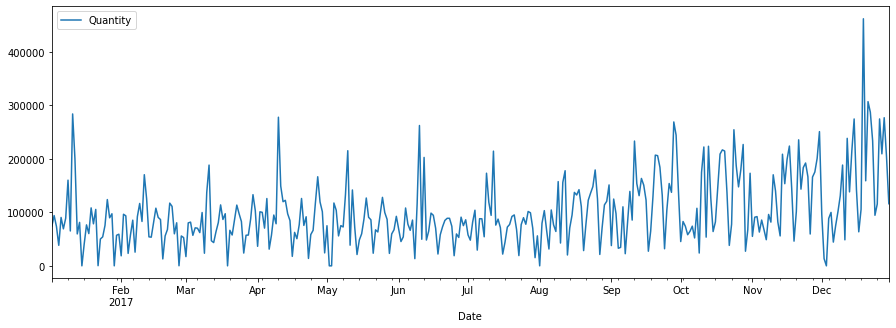
\includegraphics[width=160mm]{content/common/common.png}
        }
        \caption{Данные за 2017 год.}
        \label{img:common}
\end{figure}

Модуль \texttt{statmodels} предоставляет возможность визуально разделить временной ряд на три компоненты: тренд, сезонность и шум --- для заданного периода. Проведя серию экспериментов с разной величиной периода, было выбрано значение с визуально наименьшей выборочной дисперсией шума --- 28 дней. На рисунке Рис.~\ref{img:decomp} можно посмотреть на соответствующую декомпозицию. Также напрашивается вывод, что месячная периодичность более выражена, чем любая другая, например, недельная.

\begin{figure}[h]
        \noindent\centering{
        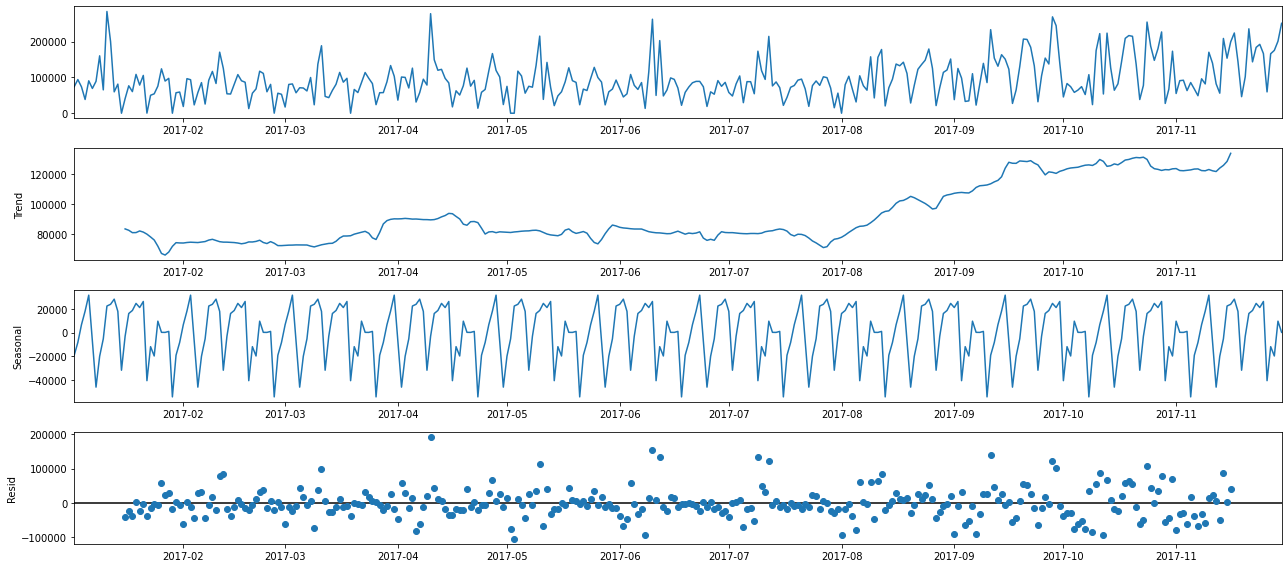
\includegraphics[width=160mm]{content/common/decomp.png}
        }
        \caption{Декомпозиция временного ряда на компоненты: тренд, сезонность и шум --- для периода в 28 дней.}
        \label{img:decomp}
\end{figure}